% LaTeX resume using res.cls
\documentclass[line,margin]{res} 
%\usepackage{helvetica} % uses helvetica postscript font (download helvetica.sty)
%\usepackage{newcent}   % uses new century schoolbook postscript font 

\newcommand{\zh}{Z\"{u}rich}
\usepackage{charter}
\usepackage{graphicx}
\usepackage{wrapfig}

\begin{document}

\name{Eivind Fonn}
% \address used twice to have two lines of address
\address{Forchstrasse 168, CH-8032 \zh}
\address{+41 78 634 68 37, evfonn@gmail.com}


\begin{resume}

\section{PERSONALIA}
    \begin{wrapfigure}{R}{0.13\textwidth}
        \vspace{-0.6cm}
        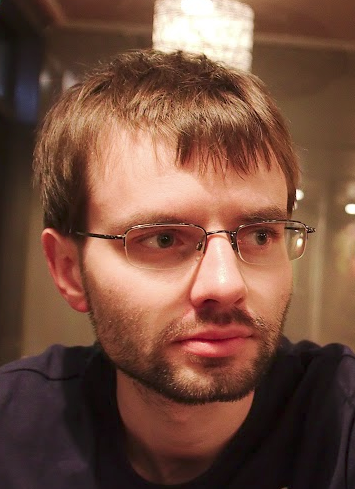
\includegraphics[width=1.5cm]{photo.png}
    \end{wrapfigure}
    I am an unmarried 29 year old Norwegian, born, grown up and with undergraduate studies in Trondheim,
    Norway. Moved to Z\"urich, Switzerland for graduate studies. Interested in mathematics, computing,
    programming, photography, chess and books. 


\section{EDUCATION} 
    {\em Ph.D.}, numerical mathematics \hfill 2009-09 $\to$ 2013-11 \\
    ETH \zh, \zh, Switzerland \\
    Solving high-dimensional kinetic transport equations, bridging the ``curse
    of dimensionality''. Particular focus on Shearlet frames and the Boltzmann
    equation.

    {\em Master of Technology}, industrial mathematics \hfill 2004-08 $\to$ 2009-06 \\
    NTNU, Trondheim, Norway \\
    Specialisation in numerical analysis and differential geometry.


\section{SKILLS}
    {\em Programming:} Python, Matlab, Haskell, C, C++, C$\sharp$, Java, PHP, JS \\
    {\em Databases:} PostgreSQL, MySQL, MS SQL \\
    {\em Assorted computer:} \LaTeX, (X)HTML, CSS, XML \\
    {\em Operating Systems:} Assorted Linux distributions, Windows \\
    {\em Languages:} Fluent Norwegian and English, decent German


\section{EXPERIENCE} 
    {\em Ph.D. student} \hfill 2009-09 $\to$ 2013-11 \\
    ETH \zh, \zh, Switzerland \\
    Solving high-dimensional kinetic transport equations, bridging the ``curse
    of dimensionality''.  Implementation in Matlab and Python. Includes a 40\%
    teaching load.

    {\em Software engineer} \hfill Summer 2009 \\
    Jeeves, Trondheim, Norway \\
    Implemented a translation tool built on Google Translate, which can read and
    write a number of different formats (such as Microsoft Word and database
    tables), with some facilities for correcting erroneous translations and
    learning.

    {\em Software engineer} \hfill Summer 2008 \\
    Yahoo! Technologies, Trondheim, Norway \\
    Implemented an adapter between MySQL and Yahoo's internal vertical search
    platform Vespa, together with several demo cases. Responsibilities included
    the entire process, from design to completion.

    {\em Scientific assistant} \hfill Summer 2007 \\
    ETH \zh, \zh, Switzerland \\
    Implemented a finite volume method for solving the
    convection/diffusion/reaction equation in Matlab. Also did some
    post-processing of photonic crystal simulations. This was an IAESTE
    internship.


\section{AWARDS}
    \begin{itemize}
        \item Winnie and Ragnar Mathisen's award for best student of technology
            or architecture in the 2009 graduating class at NTNU.
        \item The Norwegian Computing Centre's award for best master thesis in
            mathematics or ICT at NTNU in 2008/09.
        \item The Stubban award for the most promising master candidate in
            mathematics at NTNU among the 2009 graduating class.
    \end{itemize}


\section{ASSORTED}
    \begin{itemize}
        \item Founder of the Aligulac project\footnote{{\tt
            http://aligulac.com/}}, a rating system and historical database for
            professional Starcraft II, now maintained by a team of about 15
            volunteers.
        \item Part organiser of the inaugural edition of KoMiN---a now annual
            conference for mathematics students in Norway.
        \item Designed problems, graded answers and maintained the website for
            the Abel Competition, the Norwegian mathematical olympiad for high
            school students.
        \item Driving force and main organiser of the first two editions of the
            Norwegian Rubik's Cube Championship.
        \item Former national record holder in Rubik's Cube speedsolving and
            speedsolving while blindfolded (single and multiple).
    \end{itemize}


\section{POSITIONS OF TRUST}
    \begin{itemize}
        \item Webmaster\footnote{{\tt http://iaeste.ch/}} and board member for
            the IAESTE Local Comittee \zh\ for four years (2010-2013).
        \item Recognised by the World Cubing Association as a competition
            delegate.
        \item Webmaster and board member for the Student association Nabla at
            NTNU for three years (2005-2007).
    \end{itemize}


\section{REFERENCES}
    \begin{itemize}
        \item Prof. Dr. Ralf Hiptmair, Seminar for Applied Mathematics, ETH Zurich \\
            +41 44 632 34 04, ralf.hitpmair@sam.math.ethz.ch
        \item Prof. Dr. Philipp Grohs, Seminar for Applied Mathematics, ETH Zurich \\
            +41 44 632 32 00, philipp.grohs@sam.math.ethz.ch
    \end{itemize}


\section{SOCIAL SITES}
    \begin{itemize}
        \item Github: \texttt{http://github.com/TheBB}
        \item LinkedIn: \texttt{http://www.linkedin.com/pub/eivind-fonn/5/364/67}
    \end{itemize}


\end{resume}
\end{document}
